\clearpage
\setmonofont[Mapping=tex-text]{CMU Typewriter Text}
\section{Общая таблица для классов задач синтаксического анализа графов}

В данном разделе приведена таблица, содержащая существующие результаты для различных классов задач в области синтаксического анализа графов. Данные результаты были приведены к общей терминологии для упрощения таблицы.

Рассматриваемые классы задач отличаются:
\begin{itemize}
    \item семантикой запроса (поиск кратчайшего пути, простого пути и т.д.);
    \item типом входного графа (без циклов, планарный и т.д.);
    \item классом входной формальной грамматики (регулярная грамматика, контекстно-свободная и т.д.).
\end{itemize}

\begin{table}[h!]
 \centering
 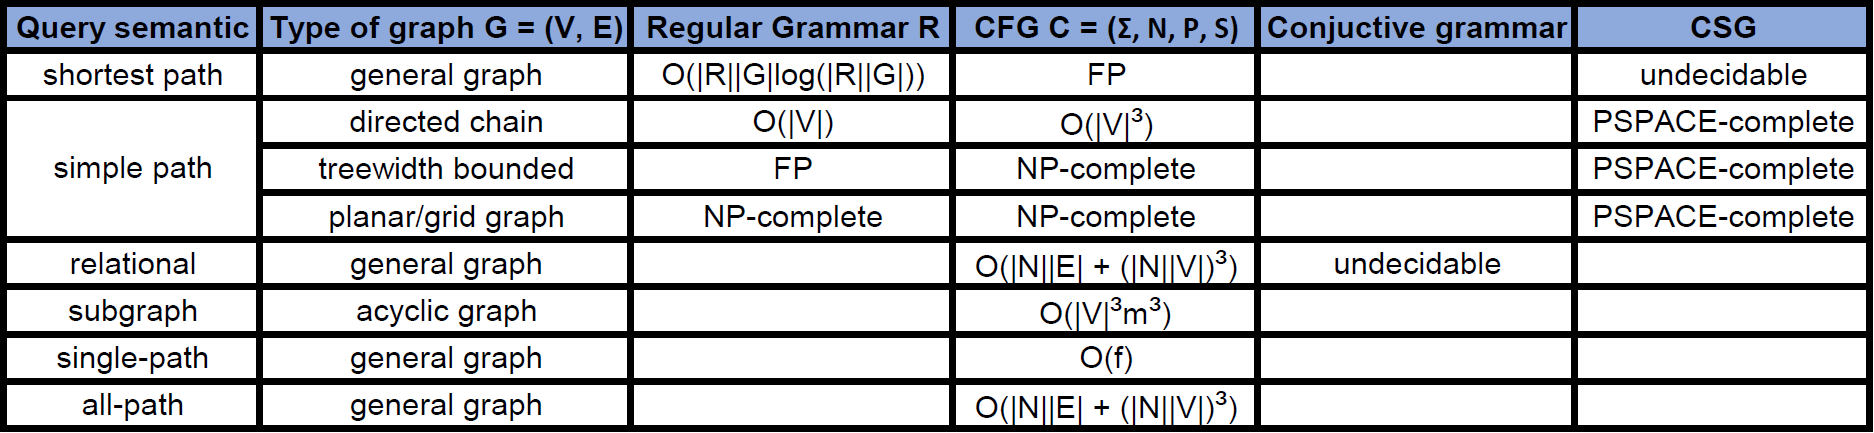
\includegraphics[width=17cm]{pictures/table_short.png}
 \caption{Общая таблица, отражающая связь классов задач синтаксического анализа графов и их характеристик. $CFG$ и $CSG$ означают контекстно-свободную и контекстно-зависимую грамматики соответственно. $FP$ означает, что искомый путь может быть найден на детерминированной машине Тьюринга за полиномиальное время, даже если спецификация формального языка является частью входных данных. $m$ означает максимальную длину пути в графе, а $f = |N||V|^{2}((|N||V|^{2}) log(|N||V|^{2}) + |P||V|^{3} + min(|N|,|P|) |E|) + 2^{|N||V|^{2} - 1}$.}
 \label{table}
\end{table}